
% SVM parameter
\newcommand{\svmT}{\bm{\theta}}
\newcommand{\svmB}{b}
\newcommand{\svmAug}{\tilde{\svmT}}
%\newcommand{\svmAugAll}{\svmAug_{\text{all}}}
\newcommand{\svmAugAll}{\bm{\Theta}}

\begin{figure}
\begin{center}
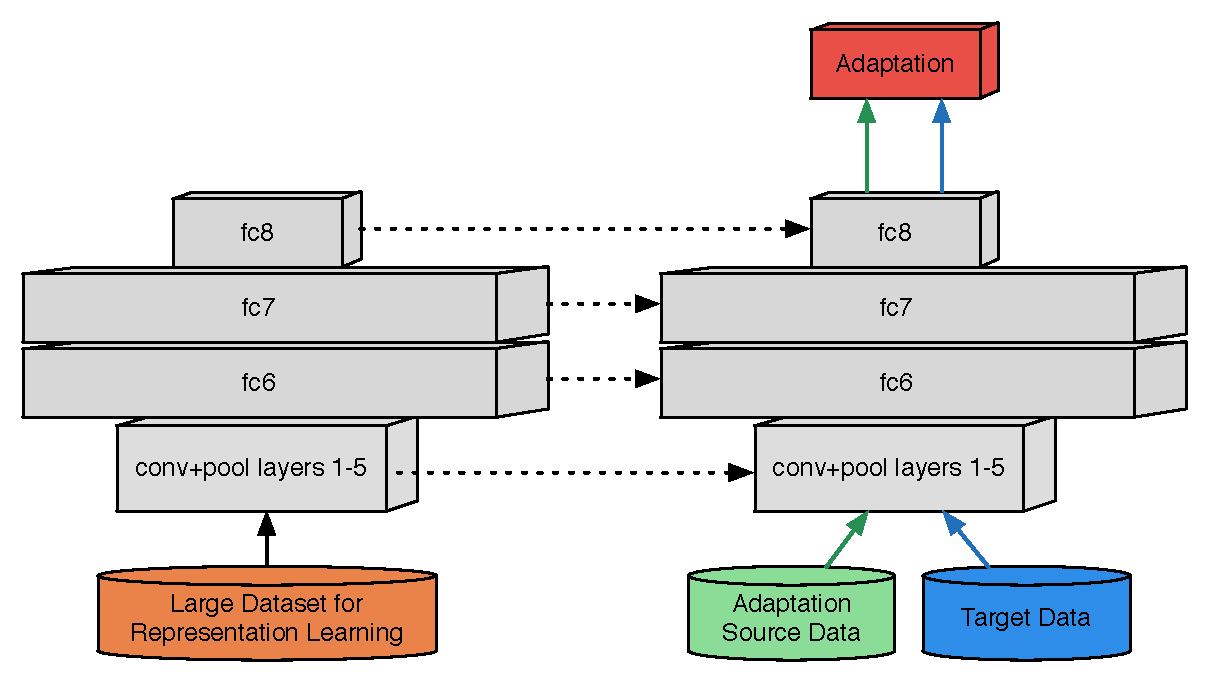
\includegraphics[width=.7\linewidth]{figs/model-adapt}
\end{center}
\caption{Our proposed adaptation model.}
\label{fig:model}
\end{figure}

% Describe adaptation algorithms
%Many methods have been proposed for visual domain adaptation. 
% \ks{similar edit as in intro, see if this make sense}

We propose a general framework for selectively adapting the parameters of a convolutional neural network (CNN) whose representation and classifier weights are trained on a large-scale source domain, such as ImageNet.
Our framework adds a final domain-adaptive classification ``layer'' that takes the activations of one of the existing network's layers as input features. Note that the network cannot be effectively fine-tuned without access to more labeled target data. This adapted layer is a linear classifier that combines source and target training data using an adaptation method. To demonstrate the generality of our framework, we select a representative set of popular linear classifier adaptation approaches that we empirically evaluate in Section~\ref{sec:eval}. We separate our discussion into the set of supervised and unsupervised adaptation settings.

Below we denote the features extracted over the source domain as $\bm{X}$ and the features extracted over the target domain as $\tilde{\bm{X}}$. Similarly, we denote the source domain image classifier as $\bm{\theta}$ and the target domain image classifier as $\bm{\tilde{\theta}}$.

\subsection{Unsupervised Adaptation}
Many unsupervised adaptation techniques seek to minimize the distance between subspaces that represent the source and target domains. We denote these subspaces as $U$ and $\tilde{U}$, respectively.

{\bf GFK~\cite{gong-cvpr12}}
The Geodesic Flow Kernel (GFK) method~\cite{gong-cvpr12} is an unsupervised domain adaptation approach which seeks embeddings for the source and target points that minimize domain shift.
Inputs to the method are $U$ and $\tilde{U}$, lower-dimensional embeddings of the source and target domains (e.g. from principal component analysis).
The method constructs the geodesic flow $\phi(t)$ along the manifold of subspaces such that $U = \phi(0)$ and $\tilde{U} = \phi(1)$.
Finally, a transformation $G$ is constructed by computing
$
G =
\int_0^1 \phi(t) \phi(t)^{\intercal} dt
$
using a closed-form solution, and classification is performed by training an SVM on the source data $\bm{X}$ and transformed target data $G\tilde{\bm{X}}$.
\\\\
{\bf SA~\cite{sa}}
The Subspace Alignment (SA) method~\cite{sa} also begins with low-dimensional embeddings of the source and target domains $U$ and $\tilde{U}$, respectively.
It seeks to minimize in $M$, a transformation matrix, the objective
$ \| UM - \tilde{U} \|^2_F$.
The analytical solution to this objective is $M^* = U^{\intercal} \tilde{U}$.
Given $M^*$, an SVM is trained on source data $\bm{X}$ and transformed target data $U M^* \tilde{U}^{\intercal} \tilde{\bm{X}}$.


\subsection{Supervised Adaptation}

{\bf Late Fusion}
Perhaps the simplest supervised adaptation method is to independently train a source and target classifier and combine the scores of the two to create a final scoring function. 
We call this approach Late Fusion. It has been explored by many for a simple adaptation approach.
Let us denote the score from the source classifier as $v_s$ and the score from the target classifier as $v_t$.  For our experiments we explore two methods of combining these scores, which are described below:
\begin{itemize}
\item {\bf Max}: Produce the scores of both the source and target classifier and simply choose the max of the two as the final score for each example. Therefore, $v_{\text{adapt}} = \max(v_s, v_t)$.
\item {\bf Linear Interpolation}: Set the score for a particular example to equal the convex combination of the source and target classifier scores,  $v_{\text{adapt}} = (1-\alpha)v_{s} + \alpha v_{t}$. This method requires setting a hyperparameter, $\alpha$, which determines the weights of the source and target classifiers.
\end{itemize}

Late Fusion has two major advantages: it is easy to implement, and the source classifier it uses may be precomputed to make adaptation very fast. In the case of the linear interpolation combination rule, however, this method can potentially suffer from having a sensitive hyperparameter. We show a hyperparameter analysis in Section~\ref{sec:eval}.

{\bf \daume~\cite{daume}}
This simple feature replication method was proposed for domain adaptation by~\cite{daume}.
The method augments feature vectors with a source component, a target component, and a shared component.
Each source data point $\bm{x}$ is augmented to $\bm{x}' = (\bm{x}; \bm{x}; \bm{0})$,
and each target data point $\tilde{\bm{x}}$ is augmented to $\tilde{\bm{x}}' = (\tilde{\bm{x}}; \bm{0}; \tilde{\bm{x}})$.
Finally, an SVM is trained on the augmented source and target data---a relatively expensive procedure given the potentially large size of the source domain and the tripled augmented feature dimensionality.

{\bf PMT~\cite{aytar-iccv11}} 
This classifier adaptation method, Projective Model Transfer (PMT), proposed by~\cite{aytar-iccv11}, is a variant of adaptive SVM. It takes as input a classifier $\svmT$ pre-trained on the source domain.
PMT-SVM learns a target domain classifier $\svmAug$ by adding an extra term to the usual SVM objective which regularizes the angle
$
\alpha(\svmAug, \svmT) =
\cos^{-1}\left(
  \frac{
    \svmT^{\intercal} \svmAug
  }{
    \| \svmT \| \| \svmAug \|
  }
\right)
$
between the target and source hyperplanes.
This results in the following loss function:
\begin{align}
\mathcal{L}_{PMT}(\svmAug)
&=
\frac{1}{2} \| \svmAug \|^2_2
+
\frac{\Gamma}{2} \| \svmAug \|^2_2 \sin^2 \alpha(\svmAug, \svmT)
+
\ell_{hinge}(\tilde{\bm{X}}, \tilde{\bm{Y}}; \svmAug)
\enspace,
\end{align}
where
$
\ell_{hinge}(\bm{X}, \bm{Y}; \svmT)
$
denotes the SVM hinge loss of a data matrix
$\bm{X}$,
label vector
$\bm{Y}$,
and classifier hyperplane $\svmT$,
and $\Gamma$ is a hyperparameter which, as it increases, enforces more transfer from the source classifier.

{\bf MMDT~\cite{hoffman-iclr13}}
% \newcommand{\mat}[1]{\begin{bmatrix} #1 \end{bmatrix}}
\newcommand{\mat}[1]{#1}
\newcommand\datransform{\mat{A}}
The Max-margin Domain Transforms (MMDT) method from~\cite{hoffman-iclr13} jointly optimizes an SVM-like objective over a feature transformation matrix $\datransform$ mapping target points to the source feature space and classifier parameters $\svmT$ in the source feature space.
In particular, MMDT minimizes the following loss function (assuming a binary classification task to simplify notation, and with
$\ell_{hinge}$
defined as in PMT):
\begin{align}
\mathcal{L}_{MMDT}(\svmT, \datransform)
&=
\frac{1}{2} \| \svmT \|^2_2
+
\frac{1}{2} \| \datransform - \mat{I} \|^2_F
+
C_s
\ell_{hinge}(\bm{X}, \bm{Y}; \svmT)
+
C_t
\ell_{hinge}(\datransform \tilde{\bm{X}}, \tilde{\bm{Y}}; \svmT)
\enspace,
\end{align}
where $C_s$ and $C_t$ are hyperparameters controlling the importance of correctly classifying the source and target points (respectively).



